\documentclass[landscape, two column, full page,reqno]{article}
\usepackage{mathrsfs}
\usepackage{amsmath,amssymb,amsthm}
\usepackage[adobe-garamond]{mathdesign}
\AtBeginDocument{%
  \let\mathbb\relax
  \DeclareMathAlphabet\PazoBB{U}{fplmbb}{m}{n}%
  \newcommand{\mathbb}{\PazoBB}%
  \let\mathcal\relax
  \DeclareMathAlphabet{\OMScal}{OMS}{cmsy}{m}{n}
  \newcommand{\mathcal}{\OMScal}%
}
\usepackage{enumitem}
\usepackage{fontspec}
\usepackage{tikz}
\usetikzlibrary{arrows}
\usepackage{multicol}
\setmainfont[Numbers={Proportional,OldStyle}]{Adobe Garamond Pro}
\usepackage{tabularx}
%NATBIB
\usepackage[comma]{natbib}
%HYPERREF PACKAGE
\usepackage{xcolor}
\PassOptionsToPackage{hyphens}{url}
\usepackage[backref=page,linktocpage=true,colorlinks]{hyperref}
\renewcommand{\backrefxxx}[3]{[\hyperlink{page.#1}{#1}]}
\hypersetup{
    colorlinks = true,
    citecolor = blue,
    urlcolor = blue,
    filecolor = blue,
    linkcolor = blue,
}
%PATCH TO ONLY HYPERLINK YEAR OF CITATION
\usepackage{etoolbox}
\makeatletter
% Patch case where name and year are separated by aysep
\patchcmd{\NAT@citex}
  {\@citea\NAT@hyper@{%
     \NAT@nmfmt{\NAT@nm}%
     \hyper@natlinkbreak{\NAT@aysep\NAT@spacechar}{\@citeb\@extra@b@citeb}%
     \NAT@date}}
  {\@citea\NAT@nmfmt{\NAT@nm}%
   \NAT@aysep\NAT@spacechar\NAT@hyper@{\NAT@date}}{}{}
% Patch case where name and year are separated by opening bracket
\patchcmd{\NAT@citex}
  {\@citea\NAT@hyper@{%
     \NAT@nmfmt{\NAT@nm}%
     \hyper@natlinkbreak{\NAT@spacechar\NAT@@open\if*#1*\else#1\NAT@spacechar\fi}%
       {\@citeb\@extra@b@citeb}%
     \NAT@date}}
  {\@citea\NAT@nmfmt{\NAT@nm}%
   \NAT@spacechar\NAT@@open\if*#1*\else#1\NAT@spacechar\fi\NAT@hyper@{\NAT@date}}
  {}{}
\makeatother
%
%Titlesec package
\usepackage{titlesec}
%Centering and readjusting size of headings
\titleformat{\section}[hang]
{\normalfont\bf\filcenter}{\thesection}{1em}{}
\titleformat{\subsection}[hang]
{\normalfont\bf\filcenter}{\thesubsection}{1em}{}
\titleformat{\subsubsection}[hang]
{\normalfont\sc\filcenter}{\thesubsubsection}{1em}{}
			% in the document preamble: 
				\let\endgraf\par % because LaTeX doesn't like \par 
			% in some command arguments 
				\let\subtitlefont\normalfont % or whatever 
				
%FOOTNOTE SPACING
\usepackage[hang,multiple,splitrule]{footmisc}
\setlength{\footnotemargin}{4mm}

\newcommand{\qd}{\begin{quote}\begin{description}  [align=left,style=nextline,leftmargin=*,labelsep=0pt,font=\normalfont]}
\newcommand{\zd}{\end{description}\end{quote}}
\newcommand{\qe}{\begin{enumerate}[align=left,style=nextline,leftmargin=17pt,labelsep=5pt,font=\normalfont]}
\newcommand{\qei}{\begin{enumerate}[align=left,style=nextline,leftmargin=15pt, labelsep=10pt,font=\normalfont]}
\newcommand{\ze}{\end{enumerate}}
\newcommand{\p}{\item}
\newcommand{\e}{\emph}
\newcommand{\mbf}{\mathbf}
\newcommand{\s}{\textsc}
\newcommand{\tbf}{\textbf}
\newcommand{\fn}{\footnote}
\newcommand{\tnot}{\neg}
\newcommand{\argu}[2]{\begin{center}\begin{minipage}{#1} \begin{enumerate}
	#2
\end{enumerate}
\end{minipage}  
\end{center}}
\newcommand{\fns}[1]{{\footnotesize #1}}
\newcommand{\qq}[1]{ ~\!^\ulcorner #1  ^\urcorner~\!}
\newcommand{\V}[1]{\llbracket #1 \rrbracket}
\newcommand{\msD}{\mathscr{D}}
\newcommand{\mcW}{\mathcal{W}}
\newcommand{\W}{\mathcal{W}}
\renewcommand{\u}{\mathfrak{u}}
\newcommand{\df}{\stackrel{\text{\tiny def}}{=}}
\newcommand{\plmodels}{\models_{\!\!\!\raisebox{-3pt}{\text{\tiny $PL$}}}}
\newcommand{\kmodels}{\models_{\!\!\!\raisebox{-3pt}{\text{\tiny$K$}}}}
\newcommand{\dmodels}{\models_{\!\!\!\raisebox{-3pt}{\text{\tiny$D$}}}}
\newcommand{\tmodels}{\models_{\!\!\!\raisebox{-3pt}{\text{\tiny$T$}}}}
\newcommand{\bmodels}{\models_{\!\!\!\raisebox{-3pt}{\text{\tiny$B$}}}}
\newcommand{\sfourmodels}{\models_{\!\!\!\raisebox{-3pt}{\text{\tiny S4}}}}
\newcommand{\sfivemodels}{\models_{\!\!\!\raisebox{-3pt}{\text{\tiny S5}}}}
\newcommand{\proves}{\mid\hspace{-3.9pt}-\hspace{3pt}}
\newcommand{\plproves}{\mid\hspace{-3.9pt}-_{\!\!\!\raisebox{-3pt}{\text{\tiny$PL$}}}\hspace{3pt}}
\newcommand{\pdproves}{\mid\hspace{-3.9pt}-_{\!\!\!\raisebox{-3pt}{\text{\tiny$PD$}}}\hspace{3pt}}
\newcommand{\kdproves}{\mid\hspace{-3.9pt}-_{\!\!\!\raisebox{-3pt}{\text{\tiny$KD$}}}\hspace{3pt}}
\newcommand{\ddproves}{\mid\hspace{-3.9pt}-_{\!\!\!\raisebox{-3pt}{\text{\tiny$DD$}}}\hspace{3pt}}
\newcommand{\tdproves}{\mid\hspace{-3.9pt}-_{\!\!\!\raisebox{-3pt}{\text{\tiny$TD$}}}\hspace{3pt}}
\newcommand{\bdproves}{\mid\hspace{-3.9pt}-_{\!\!\!\raisebox{-3pt}{\text{\tiny$BD$}}}\hspace{3pt}}
\newcommand{\sfourdproves}{\mid\hspace{-3.9pt}-_{\!\!\!\raisebox{-3pt}{\text{\tiny S4$D$}}}\hspace{3pt}}
\newcommand{\kproves}{\mid\hspace{-3.9pt}-_{\!\!\!\raisebox{-3pt}{\text{\tiny$K$}}}\hspace{3pt}}
\newcommand{\dproves}{\mid\hspace{-3.9pt}-_{\!\!\!\raisebox{-3pt}{\text{\tiny$D$}}}\hspace{3pt}}
\newcommand{\tproves}{\mid\hspace{-3.9pt}-_{\!\!\!\raisebox{-3pt}{\text{\tiny$T$}}}\hspace{3pt}}
\newcommand{\tpproves}{\mid\hspace{-3.9pt}-_{\!\!\!\raisebox{-3pt}{\text{\tiny$T^*$}}}\hspace{3pt}}
\newcommand{\bproves}{\mid\hspace{-3.9pt}-_{\!\!\!\raisebox{-3pt}{\text{\tiny$B$}}}\hspace{3pt}}
\newcommand{\bpproves}{\mid\hspace{-3.9pt}-_{\!\!\!\raisebox{-3pt}{\text{\tiny$B^*$}}}\hspace{3pt}}
\newcommand{\sfourproves}{\mid\hspace{-3.9pt}-_{\!\!\!\raisebox{-3pt}{\text{\tiny S4}}}\hspace{3pt}}
\newcommand{\sfourpproves}{\mid\hspace{-3.9pt}-_{\!\!\!\raisebox{-3pt}{\text{\tiny S4$^*$}}}\hspace{3pt}}
\newcommand{\sfiveproves}{\mid\hspace{-3.9pt}-_{\!\!\!\raisebox{-3pt}{\text{\tiny S5}}}\hspace{3pt}}
\newcommand{\sfivepproves}{\mid\hspace{-3.9pt}-_{\!\!\!\raisebox{-3pt}{\text{\tiny S5$^*$}}}\hspace{3pt}}
\newcommand{\sfivedproves}{\mid\hspace{-3.9pt}-_{\!\!\!\raisebox{-3pt}{\text{\tiny S5$D$}}}\hspace{3pt}}
\newcommand{\tbsfourproves}{\mid\hspace{-3.9pt}-_{\!\!\!\raisebox{-3pt}{\text{\tiny $T\!B$S4}}}\hspace{3pt}}
\newcommand{\dbsfourproves}{\mid\hspace{-3.9pt}-_{\!\!\!\raisebox{-3pt}{\text{\tiny $DB$S4}}}\hspace{3pt}}
\newcommand{\alf}{\phi}
\newcommand{\bet}{\psi}
\newcommand{\ff}{\leftrightarrow}
\newcommand{\otto}{\leftrightarrow}
\newcommand{\an}{\wedge}
\newcommand{\then}{\to}
\newcommand{\D}{\Diamond}
\newcommand{\B}{\Box}
\newcommand{\hs}{\hspace{2pt}}
\newcommand{\aproof}[2]{\begin{center}
\begin{tabularx}{#1}{l X l}
#2
\end{tabularx}
\end{center}}
%GRAPHICX PACKAGE
\usepackage{graphicx}
\graphicspath{{/Users/jdg83/Desktop/Figures/}}
\usepackage{xcolor}
\usepackage{fancybox}

\definecolor{ShadowColor}{RGB}{30,150,190}

\makeatletter
\newcommand\Cshadowbox{\VerbBox\@Cshadowbox}
\def\@Cshadowbox#1{%
  \setbox\@fancybox\hbox{\fbox{#1}}%
  \leavevmode\vbox{%
    \offinterlineskip
    \dimen@=\shadowsize
    \advance\dimen@ .5\fboxrule
    \hbox{\copy\@fancybox\kern.5\fboxrule\lower\shadowsize\hbox{%
      \color{gray}\vrule \@height\ht\@fancybox \@depth\dp\@fancybox \@width\dimen@}}%
    \vskip\dimexpr-\dimen@+0.5\fboxrule\relax
    \moveright\shadowsize\vbox{%
      \color{gray}\hrule \@width\wd\@fancybox \@height\dimen@}}}
\makeatother

\newcommand{\csbox}[2]{\begin{center}
\Cshadowbox{
\begin{minipage}{#1}
	#2
\end{minipage}}
\end{center}
}


\title{A Primer on Propositional Modal Logic}
\date{September 4th, 2018}
\author{M\e{{\fontspec{Minion Pro} \&}}E Core}

\usepackage{layout}
\voffset = -40pt
\textheight = 450pt
\setlength{\columnsep}{20pt}
\begin{document}
%\layout
\twocolumn[{%
 \centering
\maketitle
}]

\section{T{\footnotesize HE} L{\footnotesize ANGUAGE OF} P{\footnotesize ROPOSITIONAL} L{\footnotesize OGIC}}
\qe
\p The primitive vocabulary of propositional logic is:
	\qe
	\p Proposition letters: $P, Q, R, P_1, Q_1, R_1, \dots$
	\p Logical operators: $\neg, \to$
	\p Parenthases: $(, )$
	\ze 
\p The rules for well-formed formulae (`wffs') are as follows:
	\qe
	\p Any proposition letter is a wff.
	\p If $\qq{\phi}$ is a wff, then $\qq{\neg \phi}$ is a wff.
	\p If $\qq{\phi}$ and $\qq{\psi}$ are wffs, then $\qq{(\phi \to \psi)}$ are wffs.
	\p Nothing else is a wff.
	\ze 
\p The following are introduced as stipulative definitions:
			\begin{align*}
			(\phi \vee \psi) &\df ((\phi \to \psi) \to \psi	)	\\
			(\phi \wedge \psi) &\df \neg (\phi \to \neg \psi)	\\
			(\phi \leftrightarrow \psi) &\df \neg ((\phi \to \psi) \to \neg (\psi \to \phi))	
			\end{align*}

\section{T\fns{HE} A\fns{XIOMATIC} S\fns{YSTEM} PL}
\p Here is a simple axiomatization of classical propositional logic:
			\begin{align}
			&P \to (Q \to P)		\tag{A1}\label{1}\\
			&(P \to (Q \to R)) \to ((P \to Q) \to (P \to R))\tag{A2}\label{2}\\
			&(\neg Q \to \neg P) \to ((\neg Q \to P) \to Q)\label{3}\tag{A3}
			\end{align}
To accept these as axioms means that, at any point in an axiomatic proof, you may write down \eqref{1}, \eqref{2}, or \eqref{3}.  

In this axiomatic proof system, in addition to writing down \eqref{1}, \eqref{2}, or \eqref{3},  we are also allowed to write down anything permitted by the following two \e{rules of inference}:
		\qe
		\p[] \e{Uniform Substitution} (\e{US}): You may uniformly replace any propositional letter, $\qq{\alpha}$, occurring in a theorem of $PL$ with another wff of $PL$, $\qq{\psi}$.	
				\[
				\text{ from } \plproves \phi[\alpha_1, \alpha_2, \dots, \alpha_N] , \text{ infer } \plproves \phi [\psi_1/\alpha_1, \psi_2/\alpha_2, \dots, \psi_N/\alpha_N]
				\]
		\p[] \e{Modus Ponens} (\e{MP}): From a wff of the form $\qq{\phi \to \psi}$ and a wff of the form $\qq{\phi}$, you may infer $\qq{\psi}$.
		\ze 
\p If, by writing down the axioms \eqref{1}, \eqref{2}, and \eqref{3}, together with all of the sentences in $\Gamma$, and successively applying the rules of inference, we can eventually write down $\qq{\phi}$, then we will write
			\[
			\Gamma \plproves \phi
			\]
and we will say that $\qq{\phi}$ is \e{$PL$-provable} from the wffs in $\Gamma$.  If $\qq{\phi}$ is provable in the system $PL$ from no premises, then we say that $\qq{\phi}$ is a \e{theorem} of $PL$, and we write
			\[
			\plproves \phi
			\]
\p Here's a sample axiomatic proof establishing that $\plproves P \to P$:

\hspace{-20pt}
\begin{tabularx}{319pt}{l X l}
1. & $\plproves (P \to (Q \to R)) \to ((P \to Q) \to (P \to R))$ 					& \eqref{2}	\\
2.& $\plproves (P \to ((P \to P) \to P)) \to ((P \to (P \to P)) \to (P \to P))$			&	1 \eqref{us}	\\
3.& $\plproves P \to (Q \to P)$					&\eqref{1}	\\
4. & $\plproves P \to ((P \to P) \to P)$	& 3 \eqref{us}	\\
5. & $\plproves (P \to (P \to P)) \to (P \to P)$				& 2, 4 ($MP$)\\
6. & $\plproves P \to (P \to P)$							& 3  \eqref{us} \\
7. & $\plproves P \to P$								&5, 6  ($MP$)
\end{tabularx}


\subsection{S\fns{EMANTICS} F\fns{OR} PL}
\p An \e{interpretation function} $\V{~}$ is a function from wffs of $PL$ to $\{ 0, 1 \}$.
	\qe
	\p We require that an interpretation satisfy the following conditions:
			\qe
			\p[($\neg$)] $\V{\neg \phi} = 1$ iff $\V{\phi} = 0$.
			\p[($\to$)] $\V{\phi \to \psi} = 1$ iff $\V{\phi} = 0$ or $\V{\psi} = 1$.
			\ze 
	\ze 
\p We say that $\qq{\phi}$ is a $PL$-consequence of a set of wffs $\Gamma$, or that the argument from $\Gamma$ to $\qq{\phi}$ is $PL$-valid, written
		\[
		\Gamma \plmodels \phi
		\]
iff there is no $PL$-interpretation $\V{~}$ such that $\V{\gamma} =1$ for every $\gamma \in \Gamma$, yet $\V{\phi} = 0$.  Or, equivalently, iff, for every interpretation on which all of the premises in $\Gamma$ are true, $\qq{\phi}$ is true as well.

\p Here's an interesting and unexpected and fantastic fact: $\qq{\phi}$ is $PL$-\e{provable} from $\Gamma$ iff the argument from $\Gamma$ to $\qq{\phi}$ is $PL$-valid:
		\[
		\Gamma \plproves \phi \qquad\text{ if and only if }\qquad \Gamma \plmodels \phi
		\]
		
\section{T\fns{HE} L\fns{ANGUAGE OF} P\fns{ROPOSITIONAL} M\fns{ODAL} L\fns{OGIC}}
\p The primitive vocabulary of propositional modal logic is exactly the language of propositional logic, plus one additional logical operator, $\B$.
\p We add the following to our rules for well-formed formulae from propositional logic:
	\qe
	\p If $\qq{\phi}$ is a wff, then  $\qq{\B \phi}$ is a wff.
	\ze 
\p And we introduce the additional stipulative definition:
			\begin{align*}
			\D \phi &\df \neg \B \neg \phi
			\end{align*}

\section{T\fns{HE} S\fns{YSTEM} K}
\p The axiomatic system $K$ is characterized by one additional axiom, $K$ (the distribution axiom), and one additional rule of inference, $N$ (the rule of necessitation).  
		\[\begin{aligned}
		K \hs &: \hs \B( P \to Q) \to (\B P \to \B Q)	\\
		N \hs &: \hs \mbox{ from } \kproves \phi, \mbox{ infer } \kproves \B \phi
		\end{aligned}\]
If we add $K$ and $N$ to the axioms and rules of inference for $PL$, we get the axiomatic system $K$.  Since we know that every  theorem of $PL$ can be proven from the axioms and rules of inference for $PL$, we can make our axiomatic system $K$ a bit easier to work with by allowing ourselves to write down, as an axiom, \e{any} theorem of $PL$, and allowing ourselves to appeal to \e{any} valid $PL$ rule of inference.  Then, the axiomatic system $K$ will have the following axioms:
		\begin{align}
		& \kproves \phi, \text{ for all theorems of $PL$, $\qq{\phi}$ }			\tag{$PLT$}\label{plt}	\\
		& \kproves\B( P \to Q) \to (\B P \to \B Q)	\tag{$K$}\label{k}
		 \end{align}
And the following rules of inference:
		\begin{align}
		&\text{ all valid $PL$ inferences} 	\tag{$PLR$}\label{plr}	\\
		&\text{ from } \kproves \phi[\alpha_1, \alpha_2, \dots, \alpha_N] , \text{ infer } \kproves \phi [\psi_1/\alpha_1, \psi_2/\alpha_2, \dots, \psi_N/\alpha_N]	\tag{$US$}\label{us}\\
		& \mbox{ from } \kproves \phi, \mbox{ infer } \kproves \B \phi \tag{$N$}\label{n}
		\end{align}
\eqref{plr} allows you to appeal to \e{any} $PL$-valid rule of inference. 
\p If $\qq{\phi}$ is provable in the system $K$ from the premises in $\Gamma$, then we write
		\[
		\Gamma \kproves \phi
		\]
If $\qq{\phi}$ is provable in the system $K$ from no premises, then we say that $\qq{\phi}$ is a \e{theorem} of $K$, and we write
		\[
		\kproves \phi
		\]
\p Here is a proof schema establishing that a wff of the form $\qq{\neg \D \phi}$ is equivalent to a wff of the form $\qq{\B \neg \phi}$:
	\aproof{200pt}{
	1) & $\kproves \neg \neg P \leftrightarrow P$		&	\eqref{plt}	\\
	2)	&	$\kproves \neg \neg \B \neg \phi \leftrightarrow \B \neg \phi$	&	1 \eqref{us}	\\
	3) & $\kproves \neg \D \phi \leftrightarrow \B \neg \phi$			&	2 \e{def}.~`$\D$'
	}
We may similarly establish that a wff of the form $\qq{\neg \B \phi}$ is equivalent to a wff of the form $\qq{\D \neg \phi}$.\footnote{ We may also prove that, if $\kproves \phi \leftrightarrow \psi$, then we may replace $\qq{\phi}$ with $\qq{\psi}$ wherever it appears.  }  Let's introduce these as \e{derived} rules of inference, which we may call `$MN$', for \e{Modal Negation}:
	\[\tag{$MN$}\label{mn}
		\begin{array}{l}
	\text{ from } \zeta[\neg \B \phi]  , \text{ infer } \zeta[\D \neg \phi] 	\\
	\text{ from } \zeta[\neg \D \phi]  , \text{ infer } \zeta[\B \neg \phi] 	\\
	\text{ from } \zeta[\B \neg \phi]  , \text{ infer } \zeta[\neg \D \phi] 	\\
	\text{ from } \zeta[ \D \neg \phi]  , \text{ infer } \zeta[\neg \B \phi] 	\\
		\end{array}
	\]
(Here $\qq{\zeta[\neg \B \phi]}$ is just any wff, $\qq{\zeta}$, which contains the wff $\qq{\neg \B \phi}$ as a sub-wff, and similarly for $\qq{\zeta[\D \neg \phi]}$, $\qq{\zeta[\neg \D \phi]}$, and $\qq{\zeta[\B \neg \phi]}$.)


\subsection{S\fns{EMANTICS} F\fns{OR} K}
\p A \e{$K$-frame} is a pair $<\W, R>$ consisting of a set of worlds $\W$, a binary relation $R \subseteq \W \times \W$ (known as the `accessibility relation'---though `$Rww^*$' is colloquially glossed as `$w$ sees $w^*$').  %An illustration of a $K$-frame is shown in figure \ref{fig:frame1}.
\begin{figure}[t]
\centering
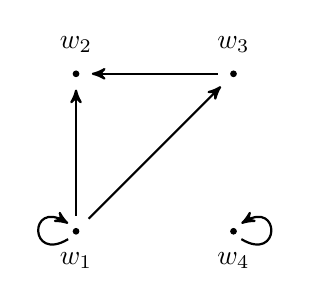
\begin{tikzpicture}[scale=2,>=stealth']
%%%WORLDS
\filldraw [black] 
(0,0) circle (0.5pt) node[anchor=north, below=4pt] { $w_1$ } 
(0, 1) circle (0.5pt)   node[anchor=south, above=4pt] { $w_2$ } 
(1,1) circle (0.5pt) node[anchor=south, above=4pt] { $w_3$ } 
(1,0) circle (0.5pt)   node[anchor=north, below=4pt] { $w_4$ } 
;
%%%ACCESSIBILITY RELATIONS 
\draw[->,thick] (0, 0.1) -- (0, 0.9);
\draw[<-, thick] (0.1,1) -- (0.9, 1);
\draw[->, thick] (0.08, 0.08) -- (0.92, 0.92);
\draw[<-, thick] (-0.05,0.05) .. controls (-0.3, 0.2) and (-0.3, -0.2) .. (-0.05, -0.05);
\draw[<-, thick] (1.05,0.05) .. controls (1.3, 0.2) and (1.3, -0.2) .. (1.05, -0.05);
\end{tikzpicture}

\caption{{\small A $K$-\e{frame} consisting of the worlds $w_1, w_2, w_3$, and $w_4$, and the accessibility relation $R$ such that $R w_1  w_1$, $R w_1 w_2$, $R w_1  w_3$, $R w_3  w_2$, and $R w_4  w_4$.}}\label{fig:frame1}
\end{figure}

\p A \e{$K$-model} is a triple $<\mathcal{W}, R, \V{~}>$ consisting of a $K$-frame and an interpretation function $\V{~}$, from pairs of wffs and worlds $w \in \mathcal{W}$ to $\{ 1, 0 \}$. 
	\qe
	\p We require that our interpretation function $\V{~}$ satisfy the following conditions:
	\qe
	\p[($\neg$)] $\V{\neg \phi}^w = 1$ iff $\V{\phi}^w = 0$.
	\p[($\to$)] $\V{\phi \to \psi}^w = 1$ iff $\V{\phi}^w = 0$ or $\V{\psi}^w = 1$.
	\p[($\B$)] $\V{\B \phi}^w = 1$ iff, for every $w^* \in \mcW$, if $R w w^*$, then $\V{\phi}^{w^*} = 1$.
	\ze
	\ze 
	\begin{figure}[t]
\centering
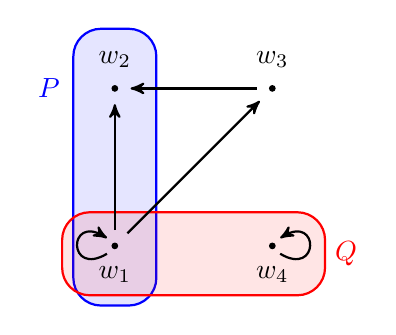
\begin{tikzpicture}[scale=2,>=stealth']
\tikzset{
    p1/.style={%
        draw=blue, thick,
        rectangle,
        rounded corners=10pt,
        minimum height=100pt,
        minimum width=30pt
        },
    q1/.style={%
        draw=red, thick,
        rectangle,
        rounded corners=10pt,
        minimum height=30pt,
        minimum width=95pt
        },
}
%%%PROPOSITIONS
\node[p1, fill=blue, fill opacity=0.1] (c2) at (0,0.5) {};
\node[q1, fill=red, fill opacity=0.1] (c1)  at (0.5,-0.05) {};
\filldraw[red]  (1.6, -0.05) node[anchor=east] { $Q$ };
\filldraw[blue]  (-0.55, 1) node[anchor=west] { $P$ };
%%%WORLDS
\filldraw [black] 
(0,0) circle (0.5pt) node[anchor=north, below=4pt] { $w_1$ } 
(0, 1) circle (0.5pt)   node[anchor=south, above=4pt] { $w_2$ } 
(1,1) circle (0.5pt) node[anchor=south, above=4pt] { $w_3$ } 
(1,0) circle (0.5pt)   node[anchor=north, below=4pt] { $w_4$ } 
;
%%%ACCESSIBILITY RELATIONS 
\draw[->,thick] (0, 0.1) -- (0, 0.9);
\draw[<-, thick] (0.1,1) -- (0.9, 1);
\draw[->, thick] (0.08, 0.08) -- (0.92, 0.92);
\draw[<-, thick] (-0.05,0.05) .. controls (-0.3, 0.2) and (-0.3, -0.2) .. (-0.05, -0.05);
\draw[<-, thick] (1.05,0.05) .. controls (1.3, 0.2) and (1.3, -0.2) .. (1.05, -0.05);
\end{tikzpicture}

\caption{{\small A \e{$K$-model} consisting of the frame from figure \ref{fig:frame1} together with an an interpretation $\V{~}$ such that $P$ is true in  $ w_1$ and  $w_2$ and $Q$ is true in  $ w_1$ and  $w_4$.\label{kmodel}}}
\end{figure}
Given this semantics for `$\neg$' and `$\Box$', it is possible to show that,  given our definition of $\qq{\D \phi}$, 
	\qe
	\p[($\D$)] $\V{\D \phi}^w = 1$ iff there is some $w^*$ such that $Rww^*$ and $\V{\phi}^{w^*}= 1$.
	\ze
 %  An illustration of a $K$-model is displayed in figure \ref{kmodel}. 


\p We will say that $\qq{\phi}$ is a $K$-consequence of a set of wffs $\Gamma$, or that the argument from $\Gamma$ to $\qq{\phi}$ is $K$-valid, written
	\[
	\Gamma \kmodels \phi
	\]
iff there is no $K$-model $< \mathcal{W}, R, \V{~} >$, with some $w \in \mathcal{W}$ such that $\V{\gamma}^w = 1$ for every $\gamma \in \Gamma$, yet $\V{\phi}^w = 0$.  Or, equivalently: iff for every  world  in every $K$-model at which all the premises in $\Gamma$ are true, $\qq{\phi}$ is true as well.


\p Here's an interesting and unexpected and fantastic fact: $\qq{\phi}$ is $K$-provable from the premises in  $\Gamma$ iff the argument from $\Gamma$ to $\qq{\phi}$ is $K$-valid.
			\[
			\Gamma \kproves \phi \quad \mbox{ if and only if } \quad \Gamma \kmodels \phi
			\]
\p Notice that, in the $K$-model shown in figure \ref{kmodel}, the wff `$\B P \to \D P$' is false at world $w_2$.  (All of the none of the worlds which $w_2$ sees are $P$-worlds, so $\V{\B P}^{w_2} = 1$.  Yet there is no world which $w_2$ sees which is a $P$-world, so $\V{ \D P}^{w_2} = 0$.)

\section{T\fns{HE} S\fns{YSTEM} D}

\p Suppose we add to our axiomatic system  $K$ the following axiom
	\[
	D \hs:\hs \B P \to \D P 
	\]
This gives us the system ${D}$.  The system $D$ will have the following axioms:
		\begin{align}
		& \dproves \phi, \text{ for all theorems of $PL$, $\qq{\phi}$ }			\tag{$PL$}\label{plt}	\\
		& \dproves\B( P \to Q) \to (\B P \to \B Q)	\tag{$K$}\label{k}	\\
		& \dproves \B P \to \D Q				\tag{$D$} \label{d}
		 \end{align}
And the following rules of inference:
		\begin{align}
		&\text{ all $PL$ valid inferences } \tag{$PLR$}\label{plr}	\\
		&\text{ from } \dproves \phi[\alpha_1, \alpha_2, \dots, \alpha_N] , \text{ infer } \dproves \phi [\psi_1/\alpha_1, \psi_2/\alpha_2, \dots, \psi_N/\alpha_N]	\tag{$US$}\label{us}\\
		& \mbox{ from } \dproves \phi, \mbox{ infer } \dproves \B \phi \tag{$N$}\label{n}
		\end{align}
(We will still retain the \e{derived} rule of inference, \ref{mn}.)
\p Here is an axiomatic proof showing that $\dproves  \neg \D P \to \D \neg P$  (this is not a theorem in $K$).  
\begin{center}
\begin{tabularx}{300pt}{l X l}
1.& $\dproves \B P \to \D P$			&	\eqref{d}	\\
2.& $\dproves \B \neg  P \to \D \neg  P$	&1  \eqref{us}	\\
3. & $\dproves \neg \D P \to \D \neg P$	& 2 \eqref{mn}
%3.& $\dproves (P \to Q) \to (\tnot \tnot P \to Q)$	&\eqref{plt}	\\
%4. & $\dproves (\B \tnot P \to \D \tnot P) \to (\tnot\tnot\B \tnot P \to \D \tnot P)$ &3, \e{US}	\\
%3. & $\dproves \tnot\tnot\B \tnot P \to \D \tnot P$	&2  \eqref{plr}	\\
%4. & $\dproves \tnot \D P \to \D \tnot P$			&5, \e{def.~`$\D$'}
\end{tabularx}
\end{center}

\subsection{S\fns{EMANTICS} F\fns{OR} D}
Our semantics for $K$ imposed absolutely no constraints on the accessibility relation $R$.    If we require that the accessibility relation $R$ be \e{serial}---that is, that every world sees at least one (not necessarily distinct) world---then we get a semantics for the system $D$.

\p A \e{$D$-frame} is a pair $< \mathcal{W}, R >$ of a set of worlds $\mathcal{W}$ and a \e{serial} binary relation $R \subseteq \mathcal{W} \times \mathcal{W}$.  A binary relation $R$ over $\W$ is \e{serial} iff every  $w \in \W$ bears $R$ to \e{something}.
	\qd
	\p[\s{Seriality}] A binary relation $R \subseteq \mbf{A} \times \mbf{A}$ is \s{serial} iff, for all $a \in \mbf{A}$, there is some $b \in \mbf{A}$ such that $Rab$.
		\[
		\forall a \hs \exists b \hs\hs Rab
		\]
	\zd
%A sample $D$-frame is shown in figure \ref{fig:frame2}.

\begin{figure}[t]
\centering
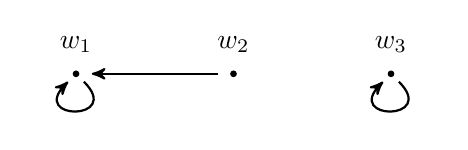
\begin{tikzpicture}[scale=2,>=stealth']
%%%WORLDS
\filldraw [black] 
(-1,0) circle (0.5pt) node[anchor=south, above=4pt] { $w_1$ } 
(0, 0) circle (0.5pt)   node[anchor=south, above=4pt] { $w_2$ } 
(1,0) circle (0.5pt) node[anchor=south, above=4pt] { $w_3$ } 
;
%%%ACCESSIBILITY RELATIONS 
\draw[->,thick] ( -0.1, 0) -- (-0.9,0);
%\draw[<-, thick] (0.1,1) -- (0.9, 1);
%\draw[->, thick] (0.08, 0.08) -- (0.92, 0.92);
\draw[<-, thick] (-1.05,-0.05) .. controls (-1.3, -0.3) and (-0.7, -0.3) .. (-0.95, -0.05);
\draw[->, thick] (1.05,-0.05) .. controls (1.3, -0.3) and (0.7, -0.3) .. (0.95, -0.05);
\end{tikzpicture}

\caption{{\small A $D$-\e{frame} consisting of the worlds $w_1, w_2,$ and  $w_3$,  and an accessibility relation $R$ such that $R w_1  w_1$, $R w_2 w_1$, and $R w_3  w_3$.}}\label{fig:frame2}
\end{figure}


\p A \e{$D$ model} is a triple $<\mathcal{W}, R, \V{~}>$ consisting of a $D$-frame $<\mathcal{W}, R>$ and an interpretation function $\V{~}$, from pairs of wffs and worlds $w \in \mathcal{W}$ to $\{ 1, 0 \}$.  
	\qe
	\p As with a $K$-model, we require that the interpretation function $\V{~}$ satisfy these constraints:
			\qe
			\p[($\neg$)] $\V{\neg \phi}^w = 1$ iff $\V{\phi}^w = 0$
			\p[($\to$)] $\V{\phi \to \psi}^w = 1$ iff $\V{\phi}^w = 0$ or $\V{\psi}^w = 1$
			\p[($\B$)] $\V{\B \phi}^w = 1$ iff $\V{\phi}^{w^*} = 1$ for all $w^*$ such that $Rww^*$.
			\ze 
	\ze 
	
	\begin{figure}[t]
\centering
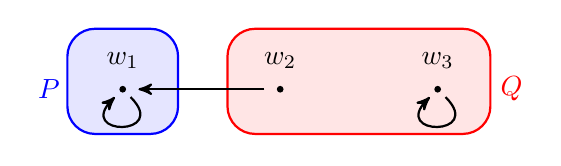
\begin{tikzpicture}[scale=2,>=stealth']
\tikzset{
    p1/.style={%
        draw=blue, thick,
        rectangle,
        rounded corners=10pt,
        minimum height=38pt,
        minimum width=40pt
        },
    q1/.style={%
        draw=red, thick,
        rectangle,
        rounded corners=10pt,
        minimum height=38pt,
        minimum width=95pt
        },
}
%%%PROPOSITIONS
\node[p1, fill=blue, fill opacity=0.1] (c2) at (-1,0.05) {};
\node[q1, fill=red, fill opacity=0.1] (c1)  at (0.5,0.05) {};
\filldraw[red]  (1.6, 0) node[anchor=east] { $Q$ };
\filldraw[blue]  (-1.6, 0) node[anchor=west] { $P$ };
%%%WORLDS
\filldraw [black] 
(-1,0) circle (0.5pt) node[anchor=south, above=4pt] { $w_1$ } 
(0, 0) circle (0.5pt)   node[anchor=south, above=4pt] { $w_2$ } 
(1,0) circle (0.5pt) node[anchor=south, above=4pt] { $w_3$ } 
;
%%%ACCESSIBILITY RELATIONS 
\draw[->,thick] ( -0.1, 0) -- (-0.9,0);
%\draw[<-, thick] (0.1,1) -- (0.9, 1);
%\draw[->, thick] (0.08, 0.08) -- (0.92, 0.92);
\draw[<-, thick] (-1.05,-0.05) .. controls (-1.3, -0.3) and (-0.7, -0.3) .. (-0.95, -0.05);
\draw[->, thick] (1.05,-0.05) .. controls (1.3, -0.3) and (0.7, -0.3) .. (0.95, -0.05);
\end{tikzpicture}

\caption{{\small A $D$-\e{model} consisting of the frame from figure \ref{fig:frame2} together with an interpretation $\V{~}$ such that $P$ is true in $w_1$ and $Q$ is true in $w_2$ and $w_3$.} }\label{dmodel}
\end{figure}

\p We will say that $\qq{\phi}$ is a $D$-consequence of a set of wffs $\Gamma$, or that the argument from $\Gamma$ to $\qq{\phi}$ is $D$-valid,
	\[
	\Gamma \dmodels \phi
	\]
iff there is no $D$-model $< \mathcal{W}, R, \V{~} >$, with some $w \in \mathcal{W}$, such that $\V{\gamma}^w = 1$ for every $\gamma \in \Gamma$, yet $\V{\phi}^w = 0$.  Or, equivalently: iff for every  world  in every $D$-model at which all the premises in $\Gamma$ are true, $\qq{\phi}$ is true as well.

\p Here's an interesting and unexpected and fantastic fact: $\qq{\phi}$ is $D$-provable from the premises in  $\Gamma$ iff the argument from $\Gamma$ to $\qq{\phi}$ is $D$-valid.
			\[
			\Gamma \dproves \phi \quad \mbox{ if and only if } \quad \Gamma \dmodels \phi
			\]
\p Notice that, in the $D$-model from figure \ref{dmodel}, `$\B P \to P$' is false at world $w_2$.  (For, at $w_2$, `$\B P$' is true---since `$P$' is true at every world that $w_2$ sees.  However, at $w_2$, `$P$' is false.  So `$\B P \to P$' is false.)

\section{T\fns{HE} S\fns{YSTEM} T}
\p Suppose we add to our axiomatic system  $K$ the following axiom
	\[
	T \hs:\hs \B P \to P
	\]
or, equivalently,	
	\[
	T^* \hs:\hs P \to \D P
	\]
	
\p This gives us the axiomatic system ${T}$.     $T$ will have the following axioms:
		\begin{align}
		& \tproves \phi, \text{ for all theorems of $PL$, $\qq{\phi}$ }			\tag{$PL$}\label{plt}	\\
		& \tproves\B( P \to Q) \to (\B P \to \B Q)	\tag{$K$}\label{k}	\\
		& \tproves \B P \to P			\tag{$T$} \label{t}	
		 \end{align}
And the following rules of inference:
		\begin{align}
		&\text{ all $PL$ valid inferences }	\tag{$PLR$}\label{plr}	\\
		&\text{ from } \tproves \phi[\alpha_1, \alpha_2, \dots, \alpha_N] , \text{ infer } \tproves \phi [\psi_1/\alpha_1, \psi_2/\alpha_2, \dots, \psi_N/\alpha_N]	\tag{$US$}\label{us}\\
		& \mbox{ from } \tproves \phi, \mbox{ infer } \tproves \B \phi \tag{$N$}\label{n}
		\end{align}
	Since all the axioms and rules of inference of $K$ are axioms and rules of inference of $T$, we retain the derived rule \eqref{mn}.
		
\p \label{31} I say that adding `$P \to \D P$' as an axiom is equivalent to adding `$\B P \to P$' as an axiom.  That's because, given this axiomatic framework, we can derive `$\B P \to P$' as a theorem if we take `$P \to \D P$' as an axiom, like so:
	\aproof{250pt}{
	1. & $\tpproves P \to \D P$				&	($T^*$)	\\
	2. & $\tpproves \neg P \to \D \neg P$		& 1 \eqref{us}	\\
	3. & $\tpproves \neg P \to \neg \B P$		& 2 \eqref{mn}	\\
	4. & $\tpproves \B P \to P$				& 3 \eqref{plr}
	}
And we can derive `$P \to \D P$' as a theorem if we take `$\B P \to P$' as an axiom, like so:
\begin{center}
\begin{tabularx}{250pt}{l X l}
1.& $\tproves \B P \to P$			&	\eqref{t}	\\
2. & $\tproves \B \neg P \to  \neg P$	& 1 \eqref{us}	\\
3. & $\tproves \neg \D P \to \neg  P$	& 2 \eqref{mn}	\\
4. & $\tproves P \to \D P$			&3, \eqref{plr}	
\end{tabularx}	
\end{center}

	
\p Notice that I did not carry over the axiom $D$, `$\B P \to \D P$'.  That is: \eqref{d} is not among the axioms for the system $T$.  The reason for this is that, given \eqref{t}, \eqref{d} is redundant.  We can derive \eqref{d} as a theorem within $T$.  To see this,  just extend the second axiomatic proof from \ref{31} above with an  application of \e{hypothetical syllogism}.
	\begin{center}
\begin{tabularx}{250pt}{l X l}
%1.& $\tproves \B P \to P$			&	\eqref{t}	\\
%$\vdots$ & $\vdots$		&	$\vdots$\\
%4.& $\tproves P \to \D P$	& 3, \eqref{plr}	\\
5. & $\tproves \B P \to \D P$							&1, 4 \eqref{plr}
\end{tabularx}	
\end{center}

\subsection{S\fns{EMANTICS} F\fns{OR} T}

If we require that the accessibility relation $R$ be \e{reflexive}---that is, that every world sees itself---then we get a semantics for the system $T$.

\p A \e{$T$-frame} is a pair $< \mathcal{W}, R >$ of a set of worlds $\mathcal{W}$ and a \e{reflexive} binary relation $R \subseteq \mathcal{W} \times \mathcal{W}$.  A relation $R$ on $\W$ is \e{reflexive} iff every $w \in \W$ bears $R$ to itself.  More generally,
	\qd
	\p[\s{reflexivity}] A binary relation $R \subseteq \mbf{A} \times \mbf{A}$ is \s{reflexive} iff, for all $a \in \mbf{A}$, $Raa$.
		\[
		\forall a \hs\hs Raa
		\]
	\zd
%A sample $T$-frame is shown in figure \ref{fig:frame3}.

\begin{figure}[t]
\centering
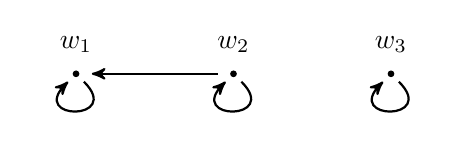
\begin{tikzpicture}[scale=2,>=stealth']
%%%WORLDS
\filldraw [black] 
(-1,0) circle (0.5pt) node[anchor=south, above=4pt] { $w_1$ } 
(0, 0) circle (0.5pt)   node[anchor=south, above=4pt] { $w_2$ } 
(1,0) circle (0.5pt) node[anchor=south, above=4pt] { $w_3$ } 
;
%%%ACCESSIBILITY RELATIONS 
\draw[->,thick] ( -0.1, 0) -- (-0.9,0);
%\draw[<-, thick] (0.1,1) -- (0.9, 1);
%\draw[->, thick] (0.08, 0.08) -- (0.92, 0.92);
\draw[<-, thick] (-1.05,-0.05) .. controls (-1.3, -0.3) and (-0.7, -0.3) .. (-0.95, -0.05);
\draw[->, thick] (1.05,-0.05) .. controls (1.3, -0.3) and (0.7, -0.3) .. (0.95, -0.05);
\draw[->, thick] (.05,-0.05) .. controls (0.3, -0.3) and (-0.3, -0.3) .. (-0.05, -0.05);
\end{tikzpicture}

\caption{\small A $T$-\e{frame} consisting of the worlds $w_1, w_2,$ and  $w_3$,  and an accessibility relation $R$ such that $R w_1  w_1$, $R w_2 w_2$, $R w_2 w_1$, and $R w_3  w_3$.}\label{fig:frame3}
\end{figure}


\p A \e{$T$-model} is a triple $<\mathcal{W}, R, \V{~}>$ consisting of a $T$-frame $<\mathcal{W}, R>$ and an interpretation function $\V{~}$, from pairs of wffs and worlds $w \in \mathcal{W}$ to $\{ 1, 0 \}$.  
	\qe
	\p As usual, we require that $\V{~}$ satisfy the following constraints.
		\qe
		\p[($\neg$)] $\V{\neg \phi}^w = 1$ iff $\V{\phi}^w = 0$.
		\p[($\to$)] $\V{\phi \to \psi}^w = 1$ iff $\V{\phi}^w = 0$ or $\V{\psi}^w = 1$.
		\p[($\B$)] $\V{\Box \phi}^w = 1$ iff, for every $w^*$ such that $R w w^*$, $\V{\phi}^{w^*}= 1$.
		\ze 		
	\ze
	
\begin{figure}[t]
\centering
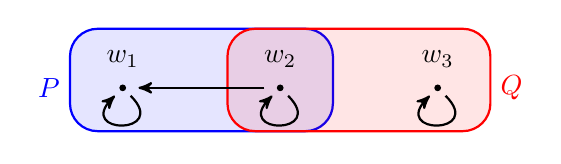
\begin{tikzpicture}[scale=2,>=stealth']
\tikzset{
    p1/.style={%
        draw=blue, thick,
        rectangle,
        rounded corners=10pt,
        minimum height=37pt,
        minimum width=95pt
        },
    q1/.style={%
        draw=red, thick,
        rectangle,
        rounded corners=10pt,
        minimum height=37pt,
        minimum width=95pt
        },
}
%%%PROPOSITIONS
\node[p1, fill=blue, fill opacity=0.1] (c2) at (-0.5,0.05) {};
\node[q1, fill=red, fill opacity=0.1] (c1)  at (0.5,0.05) {};
\filldraw[red]  (1.6, 0) node[anchor=east] { $Q$ };
\filldraw[blue]  (-1.6, 0) node[anchor=west] { $P$ };
%%%WORLDS
\filldraw [black] 
(-1,0) circle (0.5pt) node[anchor=south, above=4pt] { $w_1$ } 
(0, 0) circle (0.5pt)   node[anchor=south, above=4pt] { $w_2$ } 
(1,0) circle (0.5pt) node[anchor=south, above=4pt] { $w_3$ } 
;
%%%ACCESSIBILITY RELATIONS 
\draw[->,thick] ( -0.1, 0) -- (-0.9,0);
%\draw[<-, thick] (0.1,1) -- (0.9, 1);
%\draw[->, thick] (0.08, 0.08) -- (0.92, 0.92);
\draw[<-, thick] (-1.05,-0.05) .. controls (-1.3, -0.3) and (-0.7, -0.3) .. (-0.95, -0.05);
\draw[->, thick] (1.05,-0.05) .. controls (1.3, -0.3) and (0.7, -0.3) .. (0.95, -0.05);
\draw[->, thick] (.05,-0.05) .. controls (0.3, -0.3) and (-0.3, -0.3) .. (-0.05, -0.05);
\end{tikzpicture}
\caption{\small A $T$-\e{model} consisting of the $T$-frame from figure \ref{fig:frame3}, together with an interpretation, $\V{~}$, such that $P$ is true in  $w_1$ and $w_2$, and $Q$ is true in $w_2$ and $w_3$.}\label{tmodel}
\end{figure}

\p We will say that $\qq{\phi}$ is a $T$-consequence of a set of wffs $\Gamma$, or that the argument from $\Gamma$ to $\qq{\phi}$ is $T$-valid,
	\[
	\Gamma \tmodels \phi
	\]
iff there is no $T$-model $< \mathcal{W}, R, \V{~} >$, with some $w \in \mathcal{W}$, such that $\V{\gamma}^w = 1$ for every $\gamma \in \Gamma$, yet $\V{\phi}^w = 0$.  Or, equivalently: iff for every  world  in every $T$-model at which all the premises in $\Gamma$ are true, $\qq{\phi}$ is true as well.

\p Here's an interesting and unexpected and fantastic fact: $\qq{\phi}$ is $T$-provable from the premises in  $\Gamma$ iff the argument from $\Gamma$ to $\qq{\phi}$ is $T$-valid.
			\[
			\Gamma \tproves \phi \quad \mbox{ if and only if } \quad \Gamma \tmodels \phi
			\]
			
\section{T\fns{HE} S\fns{YSTEM} B}
\p Suppose we add to our axiomatic system  $T$ the following axiom
	\[
	B \hs:\hs  P \to \B \D P
	\]
or, equivalently,	
	\[
	B^* \hs:\hs \D \B P \to P
	\]
This gives us the axiomatic system ${B}$.     $B$ will have the following axioms:
		\begin{align}
		& \bproves \phi, \text{ for all theorems of $PL$, $\qq{\phi}$ }			\tag{$PLT$}\label{plt}	\\
		& \bproves\B( P \to Q) \to (\B P \to \B Q)	\tag{$K$}\label{k}	\\
		& \bproves \B P \to P			\tag{$T$} \label{t}			\\
		& \bproves P \to \B \D P		\tag{$B$} \label{b}
		 \end{align}
And the following rules of inference:
		\begin{align}
		&\text{ all valid $PL$ inferences }	\tag{$PLR$}\label{plr}	\\
		&\text{ from } \bproves \phi[\alpha_1, \alpha_2, \dots, \alpha_N] , \text{ infer } \bproves \phi [\psi_1/\alpha_1, \psi_2/\alpha_2, \dots, \psi_N/\alpha_N]	\tag{$US$}\label{us}\\
		& \mbox{ from } \bproves \phi, \mbox{ infer } \bproves \B \phi \tag{$N$}\label{n}
		\end{align}
	Since all the axioms and rules of inference of $K$ are axioms and rules of inference of $B$, we retain the derived rule \eqref{mn}.
		
\p I say that adding `$\D \B P \to P$' as an axiom is equivalent to adding `$P \to \B \D P$' as an axiom.  That's because, taking `$P \to \B \D P$' as an axiom, we can derive `$\D \B P \to P$', like so: 
\aproof{200pt}{
1. & $\bproves P \to \B \D P$		& 	\eqref{b}	\\
2. & $\bproves \tnot P \to \B \D \tnot P$	& 1 \eqref{us}	\\
3. &$\bproves \tnot P \to \B \tnot \B P$	& 2 \eqref{mn}	\\
4. &$\bproves \tnot P \to \tnot \D \B P$	& 3 \eqref{mn}	\\
5. &$\bproves \D \B P \to P$			& 4 \eqref{plr}
}
And  we can derive `$P \to \B\D P$' as a theorem if we take `$\D \B P \to P$' as an axiom, like so:
	\aproof{200pt}{
	1. & $\bpproves \D \B P \to P$			& ($B'$)	\\
	2. & $\bpproves \D \B \tnot P \to \tnot P$	& 1 \eqref{us}	\\
	3. & $\bpproves \D \tnot \D P \to \tnot P$	& 2 \eqref{mn}	\\
	4. & $\bpproves \tnot \B \D P \to \tnot P$	& 3 \eqref{mn}	\\
	5. & $\bpproves P \to \B \D P$			& 4 \eqref{plr}
	}
	
\subsection{S\fns{EMANTICS} F\fns{OR} B}

If we require that the accessibility relation $R$ be \e{reflexive} and \e{symmetric}---that is, that every world sees itself and every world sees all the worlds that see it---then we get a semantics for the system $B$.

\p A \e{$B$-frame} is a pair $< \mathcal{W}, R >$ of a set of worlds $\mathcal{W}$ and a \e{reflexive} and \e{symmetric} binary relation $R \subseteq \mathcal{W} \times \mathcal{W}$.  Requiring that $R$ is reflexive and symmetric means requiring that every world see itself and that, if $w$ sees $w^*$, then $w^*$ must also see $w$.  More generally,
	\qd
	\p[\s{reflexivity}] A binary relation $R \subseteq \mbf{A} \times \mbf{A}$ is \s{reflexive} iff, for all $a \in \mbf{A}$, $Raa$.
		\[
		\forall a \hs\hs Raa
		\]
	\p[\s{symmetry}] A binary relation $R \subseteq \mbf{A} \times \mbf{A}$ is \s{symmetric} iff, for all $a, b \in \mbf{A}$, if $Rab$, then $Rba$.
		\[
		\forall a \hs \forall b \hs\hs (R ab \to Rba)
		\]
	\zd
	
\begin{figure}[t]
\centering
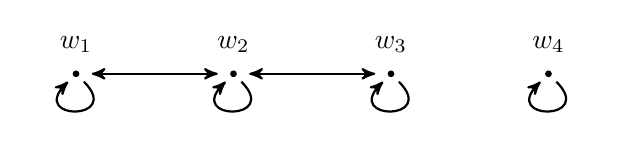
\begin{tikzpicture}[scale=2,>=stealth']
%%%WORLDS
\filldraw [black] 
(-1,0) circle (0.5pt) node[anchor=south, above=4pt] { $w_1$ } 
(0, 0) circle (0.5pt)   node[anchor=south, above=4pt] { $w_2$ } 
(1,0) circle (0.5pt) node[anchor=south, above=4pt] { $w_3$ } 
(2,0) circle (0.5pt) node[anchor=south, above=4pt] { $w_4$ } 
;
%%%ACCESSIBILITY RELATIONS 
\draw[<->,thick] ( -0.1, 0) -- (-0.9,0);
\draw[<->, thick] (0.1,0) -- (0.9, 0);
%\draw[->, thick] (0.08, 0.08) -- (0.92, 0.92);
\draw[<-, thick] (-1.05,-0.05) .. controls (-1.3, -0.3) and (-0.7, -0.3) .. (-0.95, -0.05);
\draw[->, thick] (1.05,-0.05) .. controls (1.3, -0.3) and (0.7, -0.3) .. (0.95, -0.05);
\draw[->, thick] (.05,-0.05) .. controls (0.3, -0.3) and (-0.3, -0.3) .. (-0.05, -0.05);
\draw[->, thick] (2.05,-0.05) .. controls (2.3, -0.3) and (1.7, -0.3) .. (1.95, -0.05);
\end{tikzpicture}

\caption{\small A $B$-\e{frame} consisting of the worlds $w_1, w_2,$,  $w_3$, and $w_4$, and an accessibility relation $R$ such that $R w_1  w_1$, $Rw_1w_2$, $R w_2 w_2$, $R w_2 w_1$, $Rw_2w_3$, $R w_3  w_3$, $Rw_3w_2$, and $Rw_4w_4$.}\label{fig:frame4}
\end{figure}


\p A \e{$B$-model} is a triple $<\mathcal{W}, R, \V{~}>$ consisting of a $B$-frame $<\mathcal{W}, R>$ and an interpretation function, $\V{~}$, from pairs of wffs and worlds $w \in \mathcal{W}$ to $\{ 1, 0 \}$.  
	\qe
	\p As usual, we require that $\V{~}$ satisfy the following constraints.
		\qe
		\p[($\neg$)] $\V{\neg \phi}^w = 1$ iff $\V{\phi}^w = 0$.
		\p[($\to$)] $\V{\phi \to \psi}^w = 1$ iff $\V{\phi}^w = 0$ or $\V{\psi}^w = 1$.
		\p[($\B$)] $\V{\Box \phi}^w = 1$ iff, for every $w^*$ such that $R w w^*$, $\V{\phi}^{w^*}= 1$.
		\ze 		
	\ze

\begin{figure}[t]
\centering
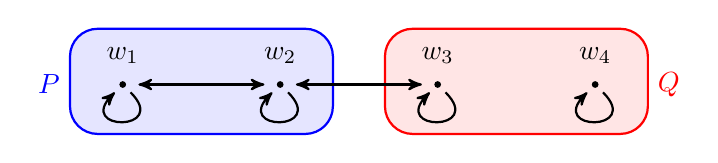
\begin{tikzpicture}[scale=2,>=stealth']
\tikzset{
    p1/.style={%
        draw=blue, thick,
        rectangle,
        rounded corners=10pt,
        minimum height=38pt,
        minimum width=95pt
        },
    q1/.style={%
        draw=red, thick,
        rectangle,
        rounded corners=10pt,
        minimum height=38pt,
        minimum width=95pt
        },
}
%%%PROPOSITIONS
\node[p1, fill=blue, fill opacity=0.1] (c2) at (-0.5,0.02) {};
\node[q1, fill=red, fill opacity=0.1] (c1)  at (1.5,0.02) {};
\filldraw[red]  (2.6, 0) node[anchor=east] { $Q$ };
\filldraw[blue]  (-1.6, 0) node[anchor=west] { $P$ };
%%%WORLDS
\filldraw [black] 
(-1,0) circle (0.5pt) node[anchor=south, above=4pt] { $w_1$ } 
(0, 0) circle (0.5pt)   node[anchor=south, above=4pt] { $w_2$ } 
(1,0) circle (0.5pt) node[anchor=south, above=4pt] { $w_3$ } 
(2,0) circle (0.5pt) node[anchor=south, above=4pt] { $w_4$ } 
;
%%%ACCESSIBILITY RELATIONS 
\draw[<->,thick] ( -0.1, 0) -- (-0.9,0);
\draw[<->, thick] (0.1,0) -- (0.9, 0);
%\draw[->, thick] (0.08, 0.08) -- (0.92, 0.92);
\draw[<-, thick] (-1.05,-0.05) .. controls (-1.3, -0.3) and (-0.7, -0.3) .. (-0.95, -0.05);
\draw[->, thick] (1.05,-0.05) .. controls (1.3, -0.3) and (0.7, -0.3) .. (0.95, -0.05);
\draw[->, thick] (.05,-0.05) .. controls (0.3, -0.3) and (-0.3, -0.3) .. (-0.05, -0.05);
\draw[->, thick] (2.05,-0.05) .. controls (2.3, -0.3) and (1.7, -0.3) .. (1.95, -0.05);
\end{tikzpicture}

\caption{\small A $B$-\e{model} consisting of the frame from figure \ref{fig:frame4}, together with an interpretation, $\V{~}$, according to which $P$ is true at $w_1$ and $w_2$, and $Q$ is true at $w_3$ and $w_4$.}\label{bmodel}
\end{figure}	
	
\p We will say that $\qq{\phi}$ is a $B$-consequence of a set of wffs $\Gamma$, or that the argument from $\Gamma$ to $\qq{\phi}$ is $B$-valid,
	\[
	\Gamma \bmodels \phi
	\]
iff there is no $B$-model $< \mathcal{W}, R, \V{~} >$, with some $w \in \mathcal{W}$, such that $\V{\gamma}^w = 1$ for every $\gamma \in \Gamma$, yet $\V{\phi}^w = 0$.  Or, equivalently: iff for every  world  in every $B$-model at which all the premises in $\Gamma$ are true, $\qq{\phi}$ is true as well.

\p Here's an interesting and unexpected and fantastic fact: $\qq{\phi}$ is $B$-provable from the premises in  $\Gamma$ iff the argument from $\Gamma$ to $\qq{\phi}$ is $B$-valid.
			\[
			\Gamma \bproves \phi \quad \mbox{ if and only if } \quad \Gamma \bmodels \phi
			\]
			
\p Notice that, in the $B$-model from figure \ref{bmodel}, `$\B P \to \B \B P$' is false at $w_1$.  (Since `$P$' is true at ever world that $w_1$ sees, `$\B P$' is true there.  However, `$\B P$' is false at $w_2$, since `$P$' is false at $w_3$, and $w_2$ sees $w_3$.  So `$\B P$' is not true at $w_2$, and is therefore not true at every world that $w_1$ sees.  So `$\B \B P$' is false at $w_1$.  So, at $w_1$, `$\B P$' is true while `$\B \B P$' is false, so `$\B P \to \B \B P$' is false at $w_1$.)
	\qe
	\p Also note that, in the same $B$-model, `$\D \D Q \to \D Q$' is false at $w_1$.  (Since $w_2$ sees a $Q$-world, `$\D Q$' is true at $w_2$.  And since $w_1$ sees $w_2$, `$\D \D Q$' is true at $w_1$.  However, $w_1$ does not see any $Q$-worlds, so `$\D Q$' is false at $w_1$.  So `$\D \D Q \to \D Q$' is false at $w_1$.)
	\ze 

\section{T\fns{HE} S\fns{YSTEM} S4}
\p Suppose we add to our axiomatic system $T$ the following axiom
	\[
	\mbox{S4} \hs:\hs \B P \to \B\B P
	\]
or, equivalently,	
	\[
	\mbox{S4}^* \hs:\hs \D \D P \to \D P
	\]
This gives us the axiomatic system {S4}.     S4 will have the following axioms:
		\begin{align}
		& \sfourproves \phi, \text{ for all theorems of $PL$, $\qq{\phi}$ }			\tag{$PL$}\label{plt}	\\
		& \sfourproves\B( P \to Q) \to (\B P \to \B Q)	\tag{$K$}\label{k}	\\
		& \sfourproves \B P \to P			\tag{$T$} \label{t}			\\
		& \sfourproves \B P \to \B \B P		\tag{S4} \label{s4}
		 \end{align}
And the following rules of inference:
		\begin{align}
		&\text{ all $PL$-valid inferences }	\tag{$PLR$}\label{plr}	\\
		&\text{ from } \sfourproves \!\phi[\alpha_1, \alpha_2, \dots, \alpha_N] , \text{ infer } \sfourproves \!\phi [\psi_1/\alpha_1, \psi_2/\alpha_2, \dots, \psi_N/\alpha_N]	\tag{$US$}\label{us}\\
		& \mbox{ from } \sfourproves \phi, \mbox{ infer } \sfourproves \B \phi \tag{$N$}\label{n}
		\end{align}
Since all the axioms and rules of inference of $K$ are axioms and rules of inference of S4, we retain the derived rule \eqref{mn}.
		\qe
		\p Notice that we \e{did not} include the axiom \eqref{b}.  Nor is \eqref{b} a theorem of this system.  For each of the previous axiomatic systems, we have been \e{enlarging} the number of theorems.  That is, for any $\qq{\phi}$ of $PML$, if $\qq{\phi}$ is a theorem of $K$, then it is a theorem of $D$; if $\qq{\phi}$ is a theorem of $D$, then it is a theorem of $T$; and if $\qq{\phi}$ is a theorem of $T$, then it is a theorem of $B$.
	\[
	\kproves \phi \hs\hs\Rightarrow\hs\hs \dproves \phi \hs\hs\Rightarrow\hs\hs \tproves \phi \hs\hs\Rightarrow\hs\hs \bproves \phi
	\]
This is not true of $B$ and S4.   Not every theorem of $B$ is a theorem of S4, 
	\[
	\bproves \phi \hs\hs\not\Rightarrow\hs\hs \sfourproves \phi
	\]
and not every theorem of S4 is a theorem of $B$
	\[
	\sfourproves \phi \hs\hs\not\Rightarrow\hs\hs \bproves \phi
	\]
%That is: $B$ and S4 are \e{logically independent}.  
Nevertheless, if $\qq{\phi}$  is a theorem of $T$, then it is a theorem of S4:
	\[
	\kproves \phi \hs\hs\Rightarrow\hs\hs \dproves \phi \hs\hs\Rightarrow\hs\hs \tproves \phi \hs\hs\Rightarrow\hs\hs \sfourproves \phi
	\]
	\ze 
		
\p I say that adding `$\D \D P \to \D P$' as an axiom is equivalent to adding `$\B P \to \B \B P$' as an axiom.  That's because, given this axiomatic framework, we can derive `$\D \D P \to \D P$' as a theorem if we take  `$\B P \to \B \B P$' as an axiom, as follows:
		\aproof{250pt}{
		1. & $\sfourproves \B P \to \B \B P$			& \eqref{s4}	\\
		2. & $\sfourproves \B \tnot P \to \B \B \tnot P$	& 1 \eqref{us}	\\
		3. & $\sfourproves \tnot \D P \to \B \tnot \D P$	& 2 \eqref{mn}	\\
		4. & $\sfourproves \tnot \D P \to \tnot \D \D P$	& 3 \eqref{mn}	\\
		5. & $\sfourproves \D \D P \to \D P$			& 4 \eqref{plr}
		}
And we can derive `$\B P \to \B\B P$' as a theorem if we take `$\D\D P \to \D P$' as an axiom:
\aproof{250pt}{
1. & $\sfourpproves \D\D P \to \D P$				& (S4$^*$)	\\
2. & $\sfourpproves \D \D \tnot P \to \D \tnot P$		& 1 \eqref{us}	\\
3. & $\sfourpproves \D \tnot \B P \to \tnot \B P$		& 2 \eqref{mn}	\\
4. & $\sfourpproves \tnot \B \B P \to \tnot \B P$		& 3 \eqref{mn}	\\
5. & $\sfourpproves \B P \to \B \B P$				& 4 \eqref{plr}
}

\subsection{S\fns{EMANTICS} F\fns{OR} S4}
If we require that the accessibility relation $R$ be \e{reflexive} and \e{transitive}---that is, that every world sees itself and every world sees the worlds seen by  the worlds it sees---then we get a semantics for the system S4.

\p An \e{S4-frame} is a pair $< \mathcal{W}, R >$ of a set of worlds $\mathcal{W}$ and a \e{reflexive} and \e{transitive} binary relation $R \subseteq \mathcal{W} \times \mathcal{W}$.  Requiring that $R$ is reflexive and transitive means requiring that every world see itself and that, if $w$ sees $w^*$, and $w^*$ sees $w^{**}$, then $w$ must also see $w^{**}$.  More generally,
	\qd
	\p[\s{reflexivity}] A binary relation $R \subseteq \mbf{A} \times \mbf{A}$ is \s{reflexive} iff, for all $a \in \mbf{A}$, $Raa$.
		\[
		\forall a \hs\hs Raa
		\]
	\p[\s{transitivity}] A binary relation $R \subseteq \mbf{A} \times \mbf{A}$ is \s{transitive} iff, for all $a, b, c \in \mbf{A}$, if $Rab$ and $Rbc$, then $Rac$.
		\[
		\forall a \hs \forall b \hs \forall c \hs\hs ((R ab \wedge Rbc) \to Rac)
		\]
	\zd

\begin{figure}[t]
\centering
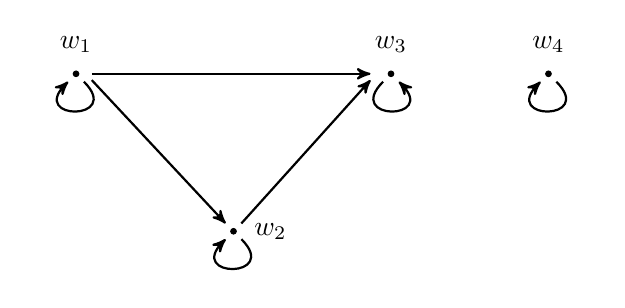
\begin{tikzpicture}[scale=2,>=stealth']
%%%WORLDS
\filldraw [black] 
(-1,0) circle (0.5pt) node[anchor=south, above=4pt] { $w_1$ } 
(0, -1) circle (0.5pt)   node[anchor=west, right=4pt] { $w_2$ } 
(1,0) circle (0.5pt) node[anchor=south, above=4pt] { $w_3$ } 
(2,0) circle (0.5pt) node[anchor=south, above=4pt] { $w_4$ } 
;
%%%ACCESSIBILITY RELATIONS 
\draw[<-,thick] ( -0.05, -0.95) -- (-0.9,-0.04);
\draw[->, thick] (0.05,-0.95) -- (0.87, -0.04);
\draw[->, thick] (-0.9,0) -- (0.87, 0);
%\draw[->, thick] (0.08, 0.08) -- (0.92, 0.92);
\draw[<-, thick] (-1.05,-0.05) .. controls (-1.3, -0.3) and (-0.7, -0.3) .. (-0.95, -0.05);
\draw[<-, thick] (1.05,-0.05) .. controls (1.3, -0.3) and (0.7, -0.3) .. (0.95, -0.05);
\draw[->, thick] (.05,-1.05) .. controls (0.3, -1.3) and (-0.3, -1.3) .. (-0.05, -1.05);
\draw[->, thick] (2.05,-0.05) .. controls (2.3, -0.3) and (1.7, -0.3) .. (1.95, -0.05);
\end{tikzpicture}

\caption{\small An \e{S4-frame} consisting of the worlds $w_1, w_2,$,  $w_3$, and $w_4$, and an accessibility relation $R$ such that $R w_1  w_1$, $Rw_1w_2$, $R w_2 w_2$, $R w_2 w_3$, $Rw_1w_3$, $R w_3  w_3$,  and $Rw_4w_4$.}\label{fig:frame5}
\end{figure}


\p An \e{S4-model} is a triple $<\mathcal{W}, R, \V{~}>$ consisting of an S4-frame $<\mathcal{W}, R>$ and an interpretation function $\V{~}$, from pairs of wffs and worlds $w \in \mathcal{W}$ to $\{ 1, 0 \}$.  
	\qe
	\p As usual, we require that $\V{~}$ satisfy the following constraints.
		\qe
		\p[($\neg$)] $\V{\neg \phi}^w = 1$ iff $\V{\phi}^w = 0$.
		\p[($\to$)] $\V{\phi \to \psi}^w = 1$ iff $\V{\phi}^w = 0$ or $\V{\psi}^w = 1$.
		\p[($\B$)] $\V{\Box \phi}^w = 1$ iff, for every $w^*$ such that $R w w^*$, $\V{\phi}^{w^*}= 1$.
		\ze 		
	\ze

\begin{figure}[t]
\centering
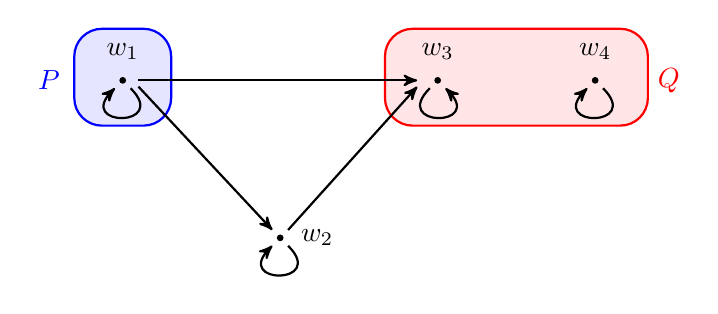
\begin{tikzpicture}[scale=2,>=stealth']
\tikzset{
    p1/.style={%
        draw=blue, thick,
        rectangle,
        rounded corners=10pt,
        minimum height=35pt,
        minimum width=35pt
        },
    q1/.style={%
        draw=red, thick,
        rectangle,
        rounded corners=10pt,
        minimum height=35pt,
        minimum width=95pt
        },
}
%%%PROPOSITIONS
\node[p1, fill=blue, fill opacity=0.1] (c2) at (-1,0.02) {};
\node[q1, fill=red, fill opacity=0.1] (c1)  at (1.5,0.02) {};
\filldraw[red]  (2.6, 0) node[anchor=east] { $Q$ };
\filldraw[blue]  (-1.6, 0) node[anchor=west] { $P$ };
%%%WORLDS
\filldraw [black] 
(-1,0) circle (0.5pt) node[anchor=south, above=4pt] { $w_1$ } 
(0, -1) circle (0.5pt)   node[anchor=west, right=4pt] { $w_2$ } 
(1,0) circle (0.5pt) node[anchor=south, above=4pt] { $w_3$ } 
(2,0) circle (0.5pt) node[anchor=south, above=4pt] { $w_4$ } 
;
%%%ACCESSIBILITY RELATIONS 
\draw[<-,thick] ( -0.05, -0.95) -- (-0.9,-0.04);
\draw[->, thick] (0.05,-0.95) -- (0.87, -0.04);
\draw[->, thick] (-0.9,0) -- (0.87, 0);
%\draw[->, thick] (0.08, 0.08) -- (0.92, 0.92);
\draw[<-, thick] (-1.05,-0.05) .. controls (-1.3, -0.3) and (-0.7, -0.3) .. (-0.95, -0.05);
\draw[<-, thick] (1.05,-0.05) .. controls (1.3, -0.3) and (0.7, -0.3) .. (0.95, -0.05);
\draw[->, thick] (.05,-1.05) .. controls (0.3, -1.3) and (-0.3, -1.3) .. (-0.05, -1.05);
\draw[->, thick] (2.05,-0.05) .. controls (2.3, -0.3) and (1.7, -0.3) .. (1.95, -0.05);
\end{tikzpicture}

\caption{\small An \e{S4-model} consisting of the frame from figure \ref{fig:frame5}, together with an interpretation on which $P$ is true at $w_1$ and $Q$ is true at $w_3$ and $w_4$.}\label{s4model}
\end{figure}	

\p We will say that $\qq{\phi}$ is an S4-consequence of a set of wffs $\Gamma$, or that the argument from $\Gamma$ to $\qq{\phi}$ is S4-valid,
	\[
	\Gamma \sfourmodels \phi
	\]
iff there is no S4-model $< \mathcal{W}, R, \V{~} >$, with some $w \in \mathcal{W}$, such that $\V{\gamma}^w = 1$ for every $\gamma \in \Gamma$, yet $\V{\phi}^w = 0$.  Or, equivalently: iff for every  world  in every S4-model at which all the premises in $\Gamma$ are true, $\qq{\phi}$ is true as well.

\p Here's an interesting and unexpected and fantastic fact: $\qq{\phi}$ is S4-provable from the premises in  $\Gamma$ iff the argument from $\Gamma$ to $\qq{\phi}$ is S4-valid.
			\[
			\Gamma \sfourproves \phi \quad \mbox{ if and only if } \quad \Gamma \sfourmodels \phi
			\]
			
\p \qe \p Note that the $B$-axiom, `$P \to \B \D P$', is false at world $w_1$ of the S4-model shown in figure \ref{s4model}.  (`$P$' is true at $w_1$.  At $w_3$, `$\D P$' is false, since $w_3$ does not see any $P$-worlds.  Since $w_1$ sees $w_3$, this means that `$\B \D P$' is false at $w_1$.  So `$P \to \B \D P$' is false at $w_1$.)
	\p Note also that, for similar reasons,  `$\D P \to \B \D P$' is false at $w_1$.
	\ze 
	
\section{T\fns{HE} S\fns{YSTEM} S5}
\p Suppose we add to our axiomatic system $T$ the following axiom
	\[
	\mbox{S5} \hs:\hs \D P \to \B\D P
	\]
or, equivalently,	
	\[
	\mbox{S5$^*$} \hs:\hs \D \B P \to \B P
	\]
This gives us the axiomatic system {S5}.     S5 will have the following axioms:
		\begin{align}
		& \sfiveproves \phi, \text{ for all theorems of $PL$, $\qq{\phi}$ }			\tag{$PL$}\label{plt}	\\
		& \sfiveproves\B( P \to Q) \to (\B P \to \B Q)	\tag{$K$}\label{k}	\\
		& \sfiveproves \B P \to P			\tag{$T$} \label{t}			\\
		& \sfiveproves \D P \to \B \D P		\tag{S5} \label{s5}
		 \end{align}
And the following rules of inference:
		\begin{align}
		&\text{ all $PL$-valid inferences }	\tag{$PLR$}\label{plr}	\\
		&\text{ from } \sfiveproves \!\phi[\alpha_1, \alpha_2, \dots, \alpha_N] , \text{ infer } \sfiveproves \!\phi [\psi_1/\alpha_1, \psi_2/\alpha_2, \dots, \psi_N/\alpha_N]	\tag{$US$}\label{us}\\
		& \mbox{ from } \sfiveproves \phi, \mbox{ infer } \sfiveproves \B \phi \tag{$N$}\label{n}
		\end{align}
Since all the axioms and rules of inference of $K$ are axioms and rules of inference of S5, we retain all the derived rule \eqref{mn}.
		
\p I say that adding the axiom `$\D \B P \to \B P$'  to $T$ is equivalent to adding `$\D P \to \B \D P$' to $T$.  That's because we can derive `$\D \B P \to \B P$' as a theorem in S5:
	\aproof{200pt}{
	1. & $\sfiveproves \D P \to \B \D P$			& \eqref{s5}	\\
	2. & $\sfiveproves \D \tnot P \to \B \D \tnot P$	& 1 \eqref{us}	\\
	3. & $\sfiveproves \tnot \B P \to \B \tnot \B P$	& 2 \eqref{mn}	\\
	4. & $\sfiveproves \tnot \B P \to \tnot \D \B P$	& 3 \eqref{mn}	\\
	5. & $\sfiveproves  \D \B P \to \B P$		& 4 \eqref{plr}
	}
And, if we take `$\D \B P \to \B P$' as an axiom, then we may derive `$\D P \to \B \D P$' as a theorem:
	\aproof{200pt}{
	1. & $\sfivepproves \D \B P \to \B  P$			& (S5$^*$)	\\
	2. & $\sfivepproves \D \B \tnot P \to \B \tnot P$	& 1 \eqref{us}	\\
	3. & $\sfivepproves \D \tnot \D P \to  \tnot \D P$	& 2 \eqref{mn}	\\
	4. & $\sfivepproves \tnot \B \D P \to \tnot \D P$	& 3 \eqref{mn}	\\
	5. & $\sfivepproves  \D P \to \B \D P$			& 4 \eqref{plr}
	}
\p Note that we didn't include either the $B$ axiom or the S4 axiom in the system S5.  However, both of these axioms are theorems of S5.  Here is a proof showing that the $B$ axiom is  a theorem in S5:
\begin{center}
\begin{tabularx}{200pt}{l X l}
%1. & $\sfiveproves \B P \to P	$			& \eqref{t}	\\
%2. & $\sfiveproves \B \tnot P \to \tnot P$		& 1 \eqref{us}	\\
%3. & $\sfiveproves \tnot \D P \to \tnot P$		& 2 \eqref{mn}	\\
1. & $\sfiveproves P \to \D P$				& ($T^*$)	\\
2. & $\sfiveproves \D P \to \B \D P$			& \eqref{s5}	\\
3. & $\sfiveproves P \to \B \D P$			& 1, 2 \eqref{plr}
\end{tabularx}	
\end{center}  
If we extend the above proof, we may derive the S4 axiom in S5:
	\aproof{200pt}{
%6. & 	$\sfiveproves P \to \B \D P$			& 4, 5 \eqref{plr}	\\
4. & $\sfiveproves \B P \to \D \B P$				& 1 \eqref{us}	\\
5. & $\sfiveproves \D \B P \to \B  P$						& (S5$^*$)		\\
6. & $\sfiveproves \B P \ff \D \B P$				& 4, 5 \eqref{plr}	\\
7. & $\sfiveproves \B P \to \B \D \B P$			& 3 \eqref{us}	\\
8. & $\sfiveproves \B P \to \B \B P$				& 6, 7 ($SE$)
	}
(On line 8, I used a rule `$SE$', for \e{substitution of equivalents}.  It says that, if $\qq{\phi \otto \psi}$ is a theorem, then $\qq{\psi}$ may be replaced for $\qq{\phi}$ wherever $\qq{\phi}$ appears as a subwff, and \e{vice versa}.  This rule is derivable in $K$.)
	\qe
	\p So both \ref{s4} and \ref{b} are redundant axioms for the system S5.  In fact, adding the \ref{s5} axiom to the system $T$ is \e{equivalent} to adding \e{both} the \ref{s4} axiom \e{and} the \ref{b} axiom to $T$.  We have already shown that adding \ref{s5} to $T$ brings along both \ref{s4} and \ref{b} as theorems.  We will now show that adding  to $T$ both the axiom \ref{s4} and the axiom \ref{b}  brings along \ref{s5} as a theorem:
	\aproof{200pt}{
	1. & $\tbsfourproves \D \D P \to \D P$			& 	\eqref{s4}	\\
	2. & $\tbsfourproves  P \to \D P$					& 	($T^*$)	\\
	3. & $\tbsfourproves \D P \to \D \D P$			& 	2 \eqref{us}	\\
	4. & $\tbsfourproves  \D P \ff \D \D P$			& 1, 3 \eqref{plr}	\\
	5. & $\tbsfourproves P \to \B \D P$				& \eqref{b}		\\
	6. & $\tbsfourproves \D P \to \B \D \D P$			& 5 \eqref{us}	\\
	7. & $\tbsfourproves \D P \to \B \D P$			& 4, 6 ($SE$)	
	}
	\ze 
	
\subsection{S\fns{EMANTICS} F\fns{OR} S5}

If we require that the accessibility relation $R$ be \e{reflexive} and \e{euclidean}---that is, that every world sees itself and all the worlds that it sees see each other---then we get a semantics for the system S5.

\p An \e{S5-frame} is a pair $< \mathcal{W}, R >$ of a set of worlds $\mathcal{W}$ and a \e{reflexive} and \e{euclidean} binary relation $R \subseteq \mathcal{W} \times \mathcal{W}$.  Requiring that $R$ is reflexive and Euclidean means requiring that every world see itself and that, if $w$ sees both $w^*$ and $w^{**}$, then $w^*$ sees $w^{**}$.  More generally,
	\qd
	\p[\s{reflexivity}] A binary relation $R \subseteq \mbf{A} \times \mbf{A}$ is \s{reflexive} iff, for all $a \in \mbf{A}$, $Raa$.
		\[
		\forall a \hs\hs Raa
		\]
	\p[\s{Euclideaness}] A binary relation $R \subseteq \mbf{A} \times \mbf{A}$ is \s{Euclidean} iff, for all $a, b, c \in \mbf{A}$, if $Rab$ and $Rac$, then $Rbc$.
		\[
		\forall a \hs \forall b \hs \forall c \hs\hs ((R ab \wedge Rac) \to Rbc)
		\]
	\zd


\begin{figure}[t]
\centering
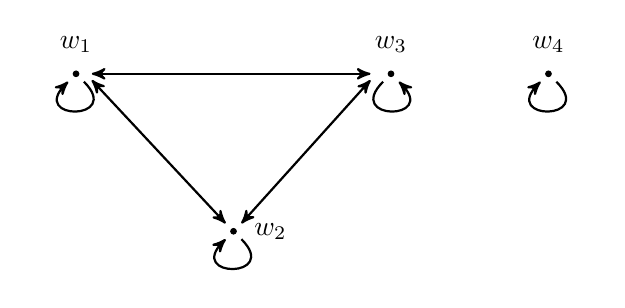
\begin{tikzpicture}[scale=2,>=stealth']
%%%WORLDS
\filldraw [black] 
(-1,0) circle (0.5pt) node[anchor=south, above=4pt] { $w_1$ } 
(0, -1) circle (0.5pt)   node[anchor=west, right=4pt] { $w_2$ } 
(1,0) circle (0.5pt) node[anchor=south, above=4pt] { $w_3$ } 
(2,0) circle (0.5pt) node[anchor=south, above=4pt] { $w_4$ } 
;
%%%ACCESSIBILITY RELATIONS 
\draw[<->,thick] ( -0.05, -0.95) -- (-0.9,-0.04);
\draw[<->, thick] (0.05,-0.95) -- (0.87, -0.04);
\draw[<->, thick] (-0.9,0) -- (0.87, 0);
%\draw[->, thick] (0.08, 0.08) -- (0.92, 0.92);
\draw[<-, thick] (-1.05,-0.05) .. controls (-1.3, -0.3) and (-0.7, -0.3) .. (-0.95, -0.05);
\draw[<-, thick] (1.05,-0.05) .. controls (1.3, -0.3) and (0.7, -0.3) .. (0.95, -0.05);
\draw[->, thick] (.05,-1.05) .. controls (0.3, -1.3) and (-0.3, -1.3) .. (-0.05, -1.05);
\draw[->, thick] (2.05,-0.05) .. controls (2.3, -0.3) and (1.7, -0.3) .. (1.95, -0.05);
\end{tikzpicture}
\caption{\small An \e{S5-frame} consisting of the worlds $w_1, w_2,$,  $w_3$, and $w_4$, and an accessibility relation $R$ such that $R w_1  w_1$, $Rw_1w_2$, $R w_1 w_3$, $R w_2 w_1$, $Rw_2w_2$, $R w_2  w_3$, $R w_3 w_1$, $Rw_3w_2$, $R w_3  w_3$, and $Rw_4w_4$.}\label{fig:frame6}
\end{figure}
\begin{figure}[t]
\centering
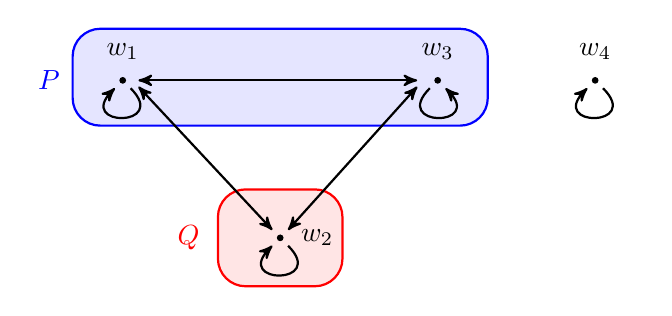
\begin{tikzpicture}[scale=2,>=stealth']
\tikzset{
    p1/.style={%
        draw=blue, thick,
        rectangle,
        rounded corners=10pt,
        minimum height=35pt,
        minimum width=150pt
        },
    q1/.style={%
        draw=red, thick,
        rectangle,
        rounded corners=10pt,
        minimum height=35pt,
        minimum width=45pt
        },
}
%%%PROPOSITIONS
\node[p1, fill=blue, fill opacity=0.1] (c2) at (0,0.02) {};
\node[q1, fill=red, fill opacity=0.1] (c1)  at (0,-1) {};
\filldraw[red]  (-0.45, -1) node[anchor=east] { $Q$ };
\filldraw[blue]  (-1.6, 0) node[anchor=west] { $P$ };
%%%WORLDS
\filldraw [black] 
(-1,0) circle (0.5pt) node[anchor=south, above=4pt] { $w_1$ } 
(0, -1) circle (0.5pt)   node[anchor=west, right=4pt] { $w_2$ } 
(1,0) circle (0.5pt) node[anchor=south, above=4pt] { $w_3$ } 
(2,0) circle (0.5pt) node[anchor=south, above=4pt] { $w_4$ } 
;
%%%ACCESSIBILITY RELATIONS 
\draw[<->,thick] ( -0.05, -0.95) -- (-0.9,-0.04);
\draw[<->, thick] (0.05,-0.95) -- (0.87, -0.04);
\draw[<->, thick] (-0.9,0) -- (0.87, 0);
%\draw[->, thick] (0.08, 0.08) -- (0.92, 0.92);
\draw[<-, thick] (-1.05,-0.05) .. controls (-1.3, -0.3) and (-0.7, -0.3) .. (-0.95, -0.05);
\draw[<-, thick] (1.05,-0.05) .. controls (1.3, -0.3) and (0.7, -0.3) .. (0.95, -0.05);
\draw[->, thick] (.05,-1.05) .. controls (0.3, -1.3) and (-0.3, -1.3) .. (-0.05, -1.05);
\draw[->, thick] (2.05,-0.05) .. controls (2.3, -0.3) and (1.7, -0.3) .. (1.95, -0.05);
\end{tikzpicture}
\caption{\small An \e{S5-model} consisting of the frame from figure \ref{fig:frame6}, together with an interpretation, $\V{~}$, according to which $P$ is true at $w_1$ and $w_3$, and $Q$ is true at $w_2$.}  \label{s5model}
\end{figure}


\p A binary relation is reflexive and Euclidean if and only if it is reflexive, symmetric, and transitive. So another, equivalent, definition of an S5-frame is this: An \e{S5-frame} is a pair $< \mathcal{W}, R >$ of a set of worlds $\mathcal{W}$ and a \e{reflexive}, \e{symmetric}, and \e{transitive} binary relation $R \subseteq \mathcal{W} \times \mathcal{W}$. 
	\qd
	\p[\s{reflexivity}] A binary relation $R \subseteq \mbf{A} \times \mbf{A}$ is \s{reflexive} iff, for all $a \in \mbf{A}$, $Raa$.
		\[
		\forall a \hs\hs Raa
		\]
	\p[\s{symmetry}] A binary relation $R \subseteq \mbf{A} \times \mbf{A}$ is \s{symmetric} iff, for all $a, b \in \mbf{A}$, if $Rab$, then $Rba$.
		\[
		\forall a \hs \forall b \hs\hs (Rab \to Rba)
		\]
	\p[\s{transitivity}] A binary relation $R \subseteq \mbf{A} \times \mbf{A}$ is \s{transitive} iff, for all $a, b, c \in \mbf{A}$, if $Rab$ and $Rbc$, then $Rac$.
		\[
		\forall a \hs \forall b \hs \forall c \hs\hs ((R ab \wedge Rbc) \to Rac)
		\]
	\zd
\p An \e{S5-model} is a triple $<\mathcal{W}, R, \V{~}>$ consisting of an S5-frame $<\mathcal{W}, R>$ and an interpretation function $\V{~}$, from pairs of wffs and worlds $w \in \mathcal{W}$ to $\{ 1, 0 \}$.  
	\qe
	\p As usual, we require that $\V{~}$ satisfy the following constraints.
		\qe
		\p[($\neg$)] $\V{\neg \phi}^w = 1$ iff $\V{\phi}^w = 0$.
		\p[($\to$)] $\V{\phi \to \psi}^w = 1$ iff $\V{\phi}^w = 0$ or $\V{\psi}^w = 1$.
		\p[($\B$)] $\V{\Box \phi}^w = 1$ iff, for every $w^*$ such that $R w w^*$, $\V{\phi}^{w^*}= 1$.
		\ze 		
	\ze

\p We will say that $\qq{\phi}$ is an S5-consequence of a set of wffs $\Gamma$, or that the argument from $\Gamma$ to $\qq{\phi}$ is S5-valid,
	\[
	\Gamma \sfivemodels \phi
	\]
iff there is no S4-model $< \mathcal{W}, R, \V{~} >$, with some $w \in \mathcal{W}$, such that $\V{\gamma}^w = 1$ for every $\gamma \in \Gamma$, yet $\V{\phi}^w = 0$.  Or, equivalently: iff for every  world  in every S5-model at which all the premises in $\Gamma$ are true, $\qq{\phi}$ is true as well.

\p Here's an interesting and unexpected and fantastic fact: $\qq{\phi}$ is S5-provable from the premises in  $\Gamma$ iff the argument from $\Gamma$ to $\qq{\phi}$ is S5-valid.
			\[
			\Gamma \sfiveproves \phi \quad \mbox{ if and only if } \quad \Gamma \sfivemodels \phi
			\]
			
			\section{S\fns{UMMARY}}
			
			\p In sum, here are the systems we've discussed characterized by the axioms they add to the system $K$, along with the constraints on the accessibility relation $R$ those axioms imply.
			\begin{center}
			\begin{tabular}{c c c c c}
			\tbf{System}		&&		\tbf{Additional Axioms}							&&		\tbf{Constraints on R}		\\\hline
			D								&&		$\B P \to \D P$					&&			$R$ is serial						\\\hline
			T								&&		$\B P \to P$							&& 			$R$ is reflexive				\\\hline
											&&     $\B P \to P$							&	&			$R$ is reflexive		\\
			B								&&		$P \to \B \D P$					&&			{\fontspec{Minion Pro} \emph{\&}} symmetric			\\
											&&		(or: $\D \B P \to P$)			&&			\\\hline
											&&		$\B P \to P$							&&			$R$ is reflexive			\\
			S4							&&		$\B  P \to \B \B P$				&&			{\fontspec{Minion Pro} \emph{\&}} transitive				\\
											&&		(or: $\D \D P \to \D P$)	&&			\\\hline
			S5							&&		$\B P \to P$				&&			$R$ is reflexive			\\
											&&		$\D P \to \B \D P$				&&			{\fontspec{Minion Pro} \emph{\&}} Euclidean		\\
											&&		(or: $\D \B P \to \B P$)									&&			\\\hline
			\end{tabular}
			\end{center}
			
			\section{R\fns{ELATIONSHIPS} B\fns{ETWEEN} T\fns{HE} S\fns{YSTEMS}}	

\p We may visualize the relationship between the logical systems we have learned with the graph from figure \ref{relationship}.
	\begin{figure}[t]
		\begin{center}
	\begin{tikzpicture}[scale = 1.5,>=stealth']
	\filldraw [black] 
(0,0) circle (0.5pt) node[anchor=east, right=3pt] { $K$ } 
(0,1) circle (0.5pt)   node[anchor=east, right=3pt] { $D$ } 
(0,2) circle (0.5pt) node[anchor=east, right=3pt] { $T$ } 
(-0.9, 3) circle (0.5pt) node[anchor=west, left = 3pt] {$B$}
(0.9, 3) circle (0.5pt) node[anchor=east, right = 3pt] {S4}
(0, 4) circle (0.5pt) node[anchor = east, right=3pt] {S5}
;
\draw[->, thick] (0, 0.1) -- (0, 0.9);
\draw[->, thick] (0, 1.1) -- (0, 1.9);
\draw[->, thick] (0, 2.1) -- (-0.8, 2.9);
\draw[->, thick] (0, 2.1) -- (0.8, 2.9);
\draw[->, thick] (-0.8, 3.1) -- (0, 3.9);
\draw[->, thick] (0.8, 3.1) -- (0, 3.9);
	\end{tikzpicture}
	\end{center}
	\caption{\small Relationship between the systems of propositional modal logic\label{relationship}.}
	\end{figure}
There, the arrows correspond to relations of \e{validity preservation}.  The graph tells us that, if an argument or a wff of $PML$ is valid in $K$, then it will be valid in $D$.  If it is valid in $D$, then it will be valid in $T$.  If it is valid in $T$, then it will be valid in $B$, and it will be valid in S4.  And, if an argument or a wff of $PML$  is valid in either $B$ or S4, then it will be  valid in S5.   

Validity-preservation is transitive, so the graph also tells us, for instance, that if an argument or wff of $PML$ is valid in $K$, then it is valid in $B$; and that, if it is valid in $D$, then it is valid in S5.
\p There are other modal systems out there.  Some of these are \e{weaker} than the system $K$.  That is, there are arguments or wffs that are valid in $K$ which are \e{not} valid in these modal logics.  Such modal logics are known as \e{non-normal} modal logics.  Any modal logic which is at least as strong as $K$ is known as a \e{normal} modal logic.  That is: any modal logic $L$ which is such that all the arguments or wffs which are valid in $K$ are valid in $L$ is  a normal modal logic.  
	\qe
	\p Even amongst the normal modal logics, there are a great many which we have not explored here.  For a taste, figure \ref{others} shows  some of the possible modal logics which we can get just from mixing and matching the modal axioms we have already seen---namely, \ref{d}, \ref{t}, \ref{b}, \ref{s4}, and \ref{s5}.    Each of the systems shown below has the axioms and rules of system $K$, plus some combination of the axioms  \ref{d}, \ref{t}, \ref{b}, \ref{s4}, and \ref{s5}.  In the figure, they are ordered in terms of validity preservation, or strength. 
 	\begin{figure}[t]
	\begin{center}
	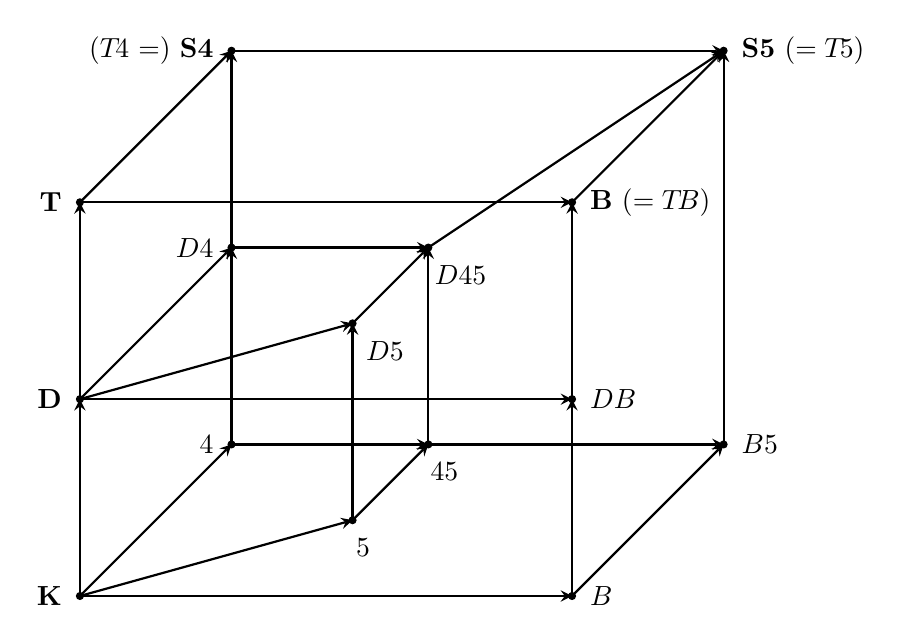
\begin{tikzpicture}[scale=2.5,>=stealth]
	\filldraw [black] 
(0,0,0) circle (0.5pt) node[anchor=east, left=3pt] { \tbf{K} } 
(0,1,0) circle (0.5pt)   node[anchor=east, left=3pt] { \tbf{D} } 
(0,2,0) circle (0.5pt) node[anchor=east, left=3pt] { \tbf{T} } 
(2.5,2,0) circle (0.5pt) node[anchor=west, right = 3pt] {\tbf{B} ($= T\!B$)}
(0, 2, -2) circle (0.5pt) node[anchor=east, left = 3pt] {$(T$\!4 $=)$ \tbf{S4}}
(2.5, 2, -2) circle (0.5pt) node[anchor = east, right=3pt] {\tbf{S5} $(= T\!$5$)$}
(0,0,-2) circle (0.5pt) node[anchor=west, left=3pt] { 4 } 
(2.5,0,0) circle (0.5pt) node[anchor=east, right=3pt] { $B$  }
(2.5,1,0) circle (0.5pt) node[anchor=east, right=3pt] { $DB$ }
(2.5,0,-2) circle (0.5pt) node[anchor=west, right=3pt] { $B$5 } 
(1,0,-1) circle (0.5pt) node[anchor=west, below=3pt] { ~\hspace{1pt} 5 } 
(1,1,-1) circle (0.5pt) node[anchor=west, below=3pt] { ~\hspace{20pt}$D$5 } 
(1,0,-2) circle (0.5pt) node[anchor=west, below=3pt] { ~\hspace{5pt} 45 }
(1,1,-2) circle (0.5pt) node[anchor=west, below=3pt] { ~\hspace{20pt}$D$45 } 
(0,1,-2) circle (0.5pt) node[anchor=east, left=3pt] { $D$4 }  
;
\draw[thick,->] (0,0,0) -- (2.5,0,0);
\draw[thick,->] (0,0,0) -- (1,0,-1);
\draw[thick,->] (1,0,-1) -- (1, 0, -2);
    \draw[thick,->] (0,0,0) -- (0,1,0);
    \draw[thick,->] (0,1,0) -- (0,2,0);
    \draw[thick,->] (0,0,0) -- (0,0,-2);
    \draw[thick,->] (2.5,0,0) -- (2.5,0,-2);
     \draw[thick,->] (0,0,-2) -- (1,0,-2);
     \draw[thick,->] (1,0,-2) -- (2.5,0,-2);
\draw[->, thick] (0,2,0)-- (0, 2, -2);
\draw[->, thick] (0,2,0) -- (2.5,2,0);
\draw[->, thick] (2.5,2,0) -- (2.5, 2, -2);
\draw[->, thick] (0, 2, -2) -- (2.5, 2, -2);
\draw[->, thick] (0,0,-2) -- (0,1,-2) ;
\draw[->, thick] (0,1,0) -- (0,1,-2);
\draw[->, thick] (0,1,-2) -- (0, 2, -2);
\draw[->, thick] (0,1,0) -- (1,1,-1);
\draw[->, thick] (1,0,-1) -- (1,1,-1);
\draw[->, thick] (1,1,-1) -- (1,1,-2);
\draw[->, thick] (0,1,-2) -- (1,1,-2);
\draw[->, thick] (1,0,-2) -- (1,1,-2);
\draw[->, thick]  (1,1,-2) -- (2.5, 2, -2);
\draw[->, thick] (2.5,0,0) -- (2.5,1,0);
\draw[->, thick] (2.5,1,0) -- (2.5,2,0);
\draw[->, thick] (0,1,0) -- (2.5,1,0);
\draw[->, thick] (2.5,0,-2) -- (2.5,2,-2);
	\end{tikzpicture}
	\end{center}
	\caption{\small Some other normal modal logics.\label{others}}
	\end{figure}

	\p In that figure, The boldfaced logics are the ones we have studied.  `$D$4' is the logic that you get if you add \ref{d} and \ref{s4} to the system $K$; `$B$5' is the logic that you get if you add \ref{b} and \ref{s5} to $K$; and so on.   For each of these normal modal logics, you may get a possible worlds semantics for the logic which is sound and complete by imposing constraints  on the accessibility relation corresponding to those axioms.  So, for instance, to get a semantics for the logic 45, you simply define  a 45-frame to be a pair $<\mcW, R>$ of a set of worlds and a binary relation $R$ which is \e{transitive} and \e{Euclidean}; and a 45-model is defined in the usual way.   
	\ze

\ze 



\end{document}
